\section{MANIFOLDS}
If $U$ and $V$ are open sets in $\F{R}^n$, a differentiable function
$h: U\to V$ with a differentiable inverse $h^{-1}:V\to U$ will be called 
a \textbf{diffeomorphism}. (``differentiable'' henceforth means ``$C^\infty$''.)

A subset $M$ of $\F{R}^n$ is called a $k$-\textbf{dimensional manifold} (in $\F{R}^n$)
if for every point $x\in M$ the following condition is satisfied:

\vspace*{1em}
\noindent($M$) There is an open set $U$ containing $x$, an open set $V\subset \F{R}^n$, and a 
diffeomorphism $h:U\to V$ such that
\begin{align*}
    h(U\cap M)
    & = V\cap (\F{R}^k\times \{0\}) \\
    & = \{y\in V:y^{k+1}=\cdots=y^n=0\}
\end{align*}

In other words, $U\cap M$ is, ``up to diffeomorphism,'' simply
$\F{R}^k\times{0}$ (see Figure \ref{Fig 5-1}). The two extreme cases of our
definition should be noted: a point in $\F{R}^n$ is a 0-dimensional
manifold, and an open subset of $\F{R}^n$ is an n-dimensional manifold.

\begin{figure}[!htb]
    \centering
    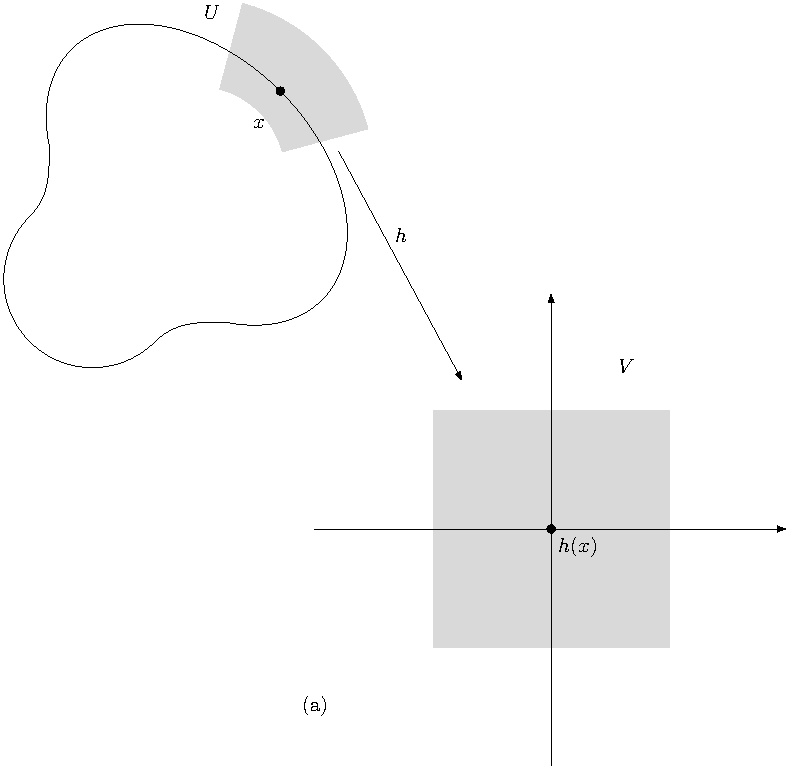
\includegraphics[width=.75\linewidth]{./pics/Fig5-1-(a).pdf}
    
    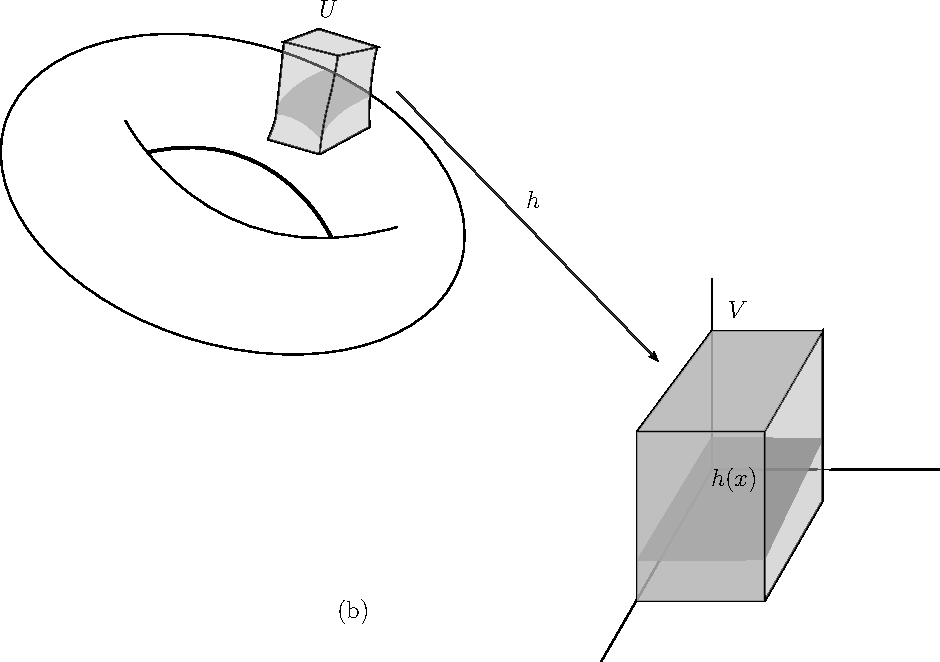
\includegraphics[width=.75\linewidth]{./pics/Fig5-1-(b).pdf}
    \caption{\textit{A one-dimensional manifold in $\F{R}^2$ and a two-dimensional manifold in $\F{R}^3$}}
    \label{Fig 5-1}
\end{figure}

One common example of an $n$-dimensional manifold is the $n$-\textbf{sphere}
$S^n$, defined as $\{x\in\F{R}^{n+1}:|x|=1\}$. We leave it as an exercise for 
the reader to prove taht condition ($M$) is satisfied. If you are unwilling 
to trouble yourself with the details, you may instead use the following theorem,
which provides many examples of manifolds (note that $S^n=g^{-1}(0)$, where $g:\F{R}^{n+1}\to\F{R}$
is defined by $g(x)=|x|^2-1$).

\begin{theorem}
    Let $A\subset \F{R}^n$ be open and let $g:A\to\F{R}^p$ be a differentiable
    function such that $g'(x)$ has $\R{rank}\; p$ whenever $g(x)=0$. Then $g^{-1}(0)$
    is an $(n-p)$-dimensional manifold in $\F{R}^n$.
\end{theorem}

\begin{proof}
    This follows immediately from Theorem 2-13. 
\end{proof}

There is an alternative characterization of manifolds which
is very important.

\begin{theorem}
    A subset $M$ of $\F{R}^n$ is a $k$-dimensional manifold if and only if for 
    each point $x\in M$ the following ``coordinate condition'' is satisfied:
    
    \vspace*{1em}
    \noindent$(C)$ There is an open set $U$ containing $x$ , an open set $W\subset\F{R}^k$,
    and a 1-1 differentiable function $f:W\to\F{R}^n$ such that
    \begin{enumerate}[label=\upshape{(\arabic*)}]
        \item $f(W)=M\cap U$.
        \item $f'(y)$ has $\R{rank}\; k$ for each $y\in W$.
        \item $f^{-1}:f(W)\to W$ is continuous.
    \end{enumerate}
\end{theorem}

[Such a function $f$ is called a \textbf{coordinate system} around $x$ (see Figure \ref{Fig 5-2}).]

\begin{figure}[!htb]
    \centering
    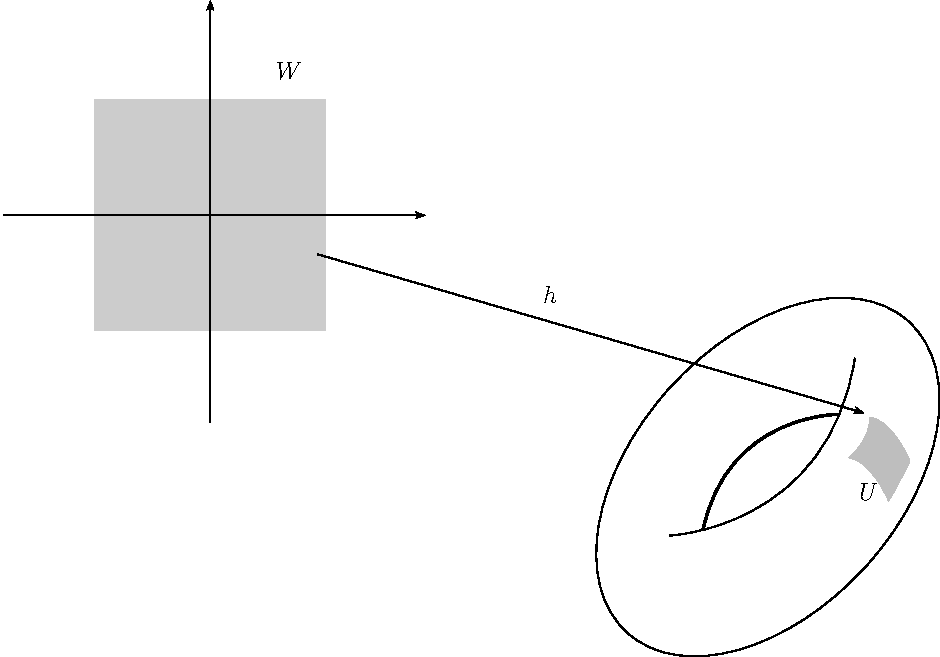
\includegraphics[width=.75\linewidth]{./pics/Fig5-2.pdf}
    \caption{}
    \label{Fig 5-2}
\end{figure}

\begin{proof}
    If $M$ is a $k$-dimensional manifold in $\F{R}^n$, choose $h:U\to V$ satisfying $(M)$. Let 
    $W=\{a\in\F{R}^k:(a,0)\in h(M)\}$ and define $f:W\to\F{R}^n$ by $f(a)=h^{-1}(a,0)$. Clearly 
    $f(W)=M\cap U$ and $f^{-1}$ is continuous. If $H:U\to\F{R}^k$ is $H(z)=(h^1(z),\cdots,h^k(z))$,
    then $H(f(y))=y$ for all $y\in W$; therefore $H'(f(y))\cdot f'(y)=I$ and $f'(y)$ must have 
    $\R{rank}\; k$.

    Suppose, conversely, that $f:W\to\F{R}^n$ satisfies condition $(C)$. Let $x=f(y)$. Assume that 
    the matrix $\R{D}_if^i(y), 1\le i,j\le k$ has a non-zero determinant. Define $g:W\times \F{R}^{n-k}\to\F{R}^n$
    by $g(a,b)=f(a)+(0,b)$. Then $\det g'(a,b)=\det(\R{D}_if^i(a))$, so $\det g'(y,0)\neq 0$. By Theorem 2-11
    there is an open set $V_1'$ containing $(y,0)$ and an open set $V_2'$ containing $g(y,0)=x$ such that
    $g:V_1'\to V_2'$ has a differentiable inverse $h:V_2'\to V_1'$. Since $f^{-1}$ is continuous, 
    $\{f(a):(a,0)\in V_1'\} = \{U\cap f(W)\}$ for some open set $U$. Let $V_2=V_2'\cap U$ and $V_1=g^{-1}(V_2)$.
    Then $V_2\cap M$ is exactly $\{f(a):(a,0)\in V_1\} = \{g(a,0):(a,0)\in V_1\}$, so 
    \begin{align*}
        h(V_1\cap M) 
        & = g^{-1}(V_1\cap M) \\
        & = g^{-1}(\{g(a,0):(a,0)\in V_1\}) \\
        & = V_1\cap (\F{R}^k\times \{0\})
    \end{align*} 
\end{proof}

One consequence of the proof of Theorem 5-2 should be noted. If $f_1:W_1\to\F{R}^n$ and 
$f_2:W_2\to \F{R}^n$ are two coordinate systems, then 
\begin{align*}
    f_2^{-1}\circ f_1:f_1^{-1}(f_2(W_2))\to \F{R}^k
\end{align*}

is differentiable with non-singular Jacobian. If fact, $f_2^{-1}(y)$ consists of the first
$k$ components of $h(y)$.

The \textbf{half-space} $\F{H}^k\in\F{R}^k$ is defined as $\{x\in\F{R}^k:x^k\ge 0\}$. A subset 
$M$ of $\F{R}^n$ is a $k$-\textbf{dimensional manifold-with-boundary} (Figure \ref{Fig 5-3}) if for evry point 
$x\in M$ either condition $(M)$ or the following condition is satisfied:

\begin{figure}[!htb]
    \centering
    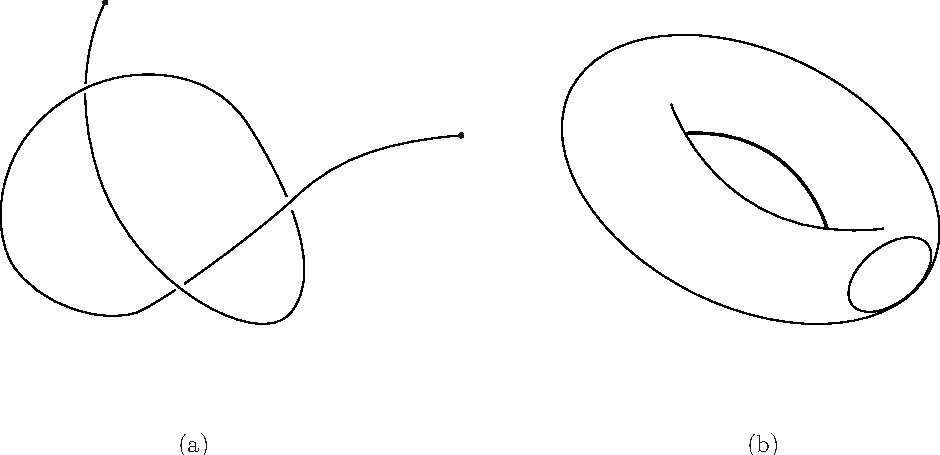
\includegraphics[width=.75\linewidth]{./pics/Fig5-3.pdf}
    \caption{}
    \label{Fig 5-3}
\end{figure}

\noindent $(M')$ is an open set $U$ containing $x$, an open set $V\in\F{R}^n$, and a diffeomorphism 
$h:U\to V$ such that 
\begin{align*}
    h(U\cap M) 
    & = V\cap(\F{H}^k\times \{0\}) \\
    & = \{y\in V:y^k\ge 0\text{ and } y^{k+1}=\cdots=y^n=0\}
\end{align*}

and $h(x)$ has $k$th component = 0.

It is important to note that condition $(M)$ and $(M')$ connot bothh hold for the same $x$. In 
fact, if $h_1:U_1\to V_1$ and $h_2:U_2\to V_2$ satisfied $(M)$ and $(M')$, respectively, then 
$h_1\circ h_2^{-1}$ would be a differentiable map that takes an open set in $\F{R}^k$, containing
$h(x)$, into a subset of $\F{H}^k$ which is not open in $\F{R}^k$. The $\det (h_2\circ h_1^{-1})'\neq 0$,
this contradicts Problem 2-36. The set of all points $x\in M$ for which condition $M'$ is satisfied
is called the \textbf{boundary} of $M$ and denoted $\partial M$. This must not be confused with the 
boundary of a set, as defined in Chapter 1 (see Problems 5-3 and 5-8).


\begin{problems}
    \problem{
        If $M$ is a $k$-dimensional manifold-with-boundary, prove that $\partial M$ 
        is a $(k-1)$-dimensional manifold and $M-\partial M$ is a $k$-dimensional manifold.
    }
    \problem{
        Find a counterexample to Theorem 5-2 if condition (3) is omitted. \textit{Hint:} 
        Wrap an open interval into a figure six.
    }
    \problem{
        \begin{enumerate}[label=(\alph*)]
            \item Let $A\subset\F{R}^n$ be an open set such that boundary $A$ is an $(n-1)$-dimensional 
                manifold. Show that $N = A \cup \text{boundary } A$ is an $n$-dimensional manifold-with-boundary.
                (It is well to bear in mind the following example: if $A = (x\in\F{R}^n: |x| < 1 \text{ or } 1 < |x| < 2\}$
                then $N = A\cup \text{boundary } A$ is a manifold-with-boundary, but $\partial N$ boundary $A$.)
            \item Prove a similar assertion for an open subset of an $n$-dimensional manifold.
        \end{enumerate}
    }
    \problem{
        Prove a partial converse of Theorem 5-1: If $M\subset \F{R}^n$ is a $k$-dimensional manifold,
        and $x\in M$, then there is an open set $A\subset \F{R}^n$ containing $x$ and a differentiable
        function $g:A\to\F{R}^{n-k}$ such that $A\cap M=g^{-1}(0)$ and $g'(y)$ has $\R{rank}\; n-k$ when 
        $g(y)=0$.
    }
    \problem{
        Prove that a $k$-dimensional (vector) subspace of $\F{R}^n$ is a $k$-dimensional manifold.
    }
    \problem{
        If $f:\F{R}^n\to\F{R}^m$, the \textbf{graph} of $f$ is $\{(x,y):y=f(x)\}$. Show that 
        the graph of $f$ is an $n$-dimensional manifold if and only if $f$ is differentiable.
    }
    \problem{
        Let $\F{K}^n=\{x\in\F{R}^n:x^1=0\text{ and } x^2,\cdots x^{n-1}>0\}$. If $M\subset \F{K}^n$
        is a $k$-dimensional manifold and $N$ is obtained by revoving $M$ around the axis $x^1=\cdots=x^{n-1}=0$,
        show that $N$ is a $(k+1)$-dimensional manifold. Example: the torus (Figure \ref{Fig 5-4}).
        \begin{figure}[!htb]
            \centering
            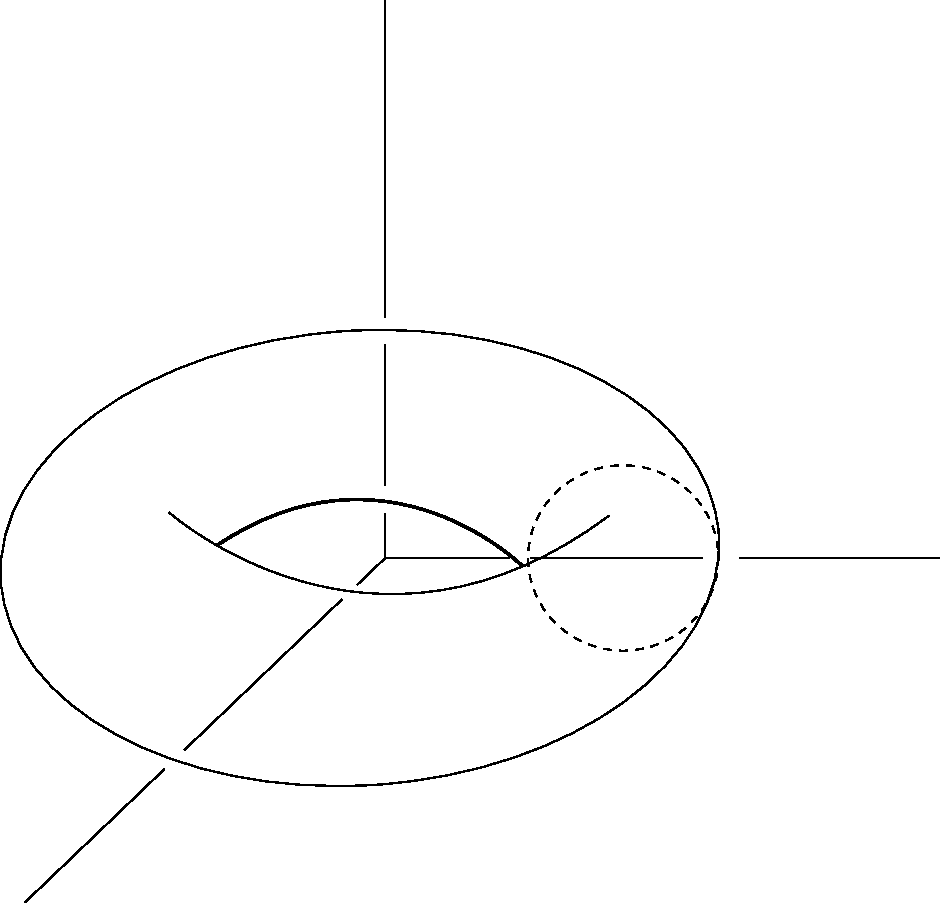
\includegraphics[width=.75\linewidth]{./pics/Fig5-4.pdf}
            \caption{}
            \label{Fig 5-4}
        \end{figure}
    }
    \problem{
        \begin{enumerate}[label=(\alph*)]
            \item If $M$ is a $k$-dimensional manifold in $\F{R}^n$ and $k < n$, show that $M$ has measure 0.
            \item If $M$ is a closed $n$-dimensional manifold-with-boundary in $\F{R}^n$, show that the boundary 
                of $M$ is $\partial M$. Give a counterlxample if $M$ is not closed.
            \item If $M$ is a compact $n$-dimensional manifold-with-boundary in $\F{R}^n$, show that $M$ is Jordan-measurable.
        \end{enumerate}
    }
\end{problems}